\EXERCISE
فرض کنید یک جدول
$n \times n$
داریم
$(n \in N)$
. خانه‌های جدول را با استفاده از اعداد حقیقی مثبت پر نموده‌ایم به قسمی که هر خانه‌ی جدول برابر با میانگین اعداد احاطه‌کننده‌ی خود باشد. ثابت کنید تمام اعداد جدول با هم مساوی هستند:
$$A = \frac{\sum_{i=1}^{8} a_i}{8}$$
\begin{center}
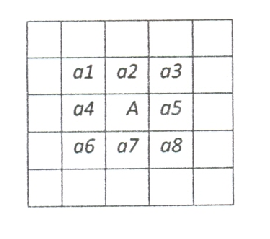
\includegraphics[height=4cm]{12.png}
\end{center}